% vim: set textwidth=78 autoindent:

\thispagestyle{empty}
\addcontentsline{toc}{section}{Authors and Contributors}

%%%%%%%%%%% nothing to change above %%%%%%%%%%

\section*{Authors and Contributors}

% when the revision of a section has been finalized, 
% comment out the following line:
%\updatedisclaimer

\begin{figure}[ht]
\begin{center}
\begin{minipage}[h]{5cm}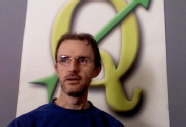
\includegraphics[width=4.7cm]{tim_sutton}
\end{minipage}
\begin{minipage}[h]{11.5cm} 
\textbf{Tim Sutton - Editor \& Lead Author} \\
Tim Sutton is a developer and project steering committee member of the
Quantum GIS project. He is passionate about seeing GIS being Freely available
to everyone. Tim is also a founding member of Linfiniti Consulting CC. - a
small business set up with the goal of helping people to learn and use open
source GIS software. \\
Web: http://linfiniti.com , Email: tim@linfiniti.com
\end{minipage}

\vspace{0.1cm}

\begin{minipage}[h]{5cm}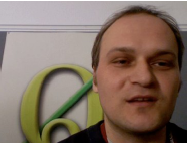
\includegraphics[width=4.7cm]{otto_dassau}
\end{minipage}
\begin{minipage}[h]{11.5cm}
\textbf{Otto Dassau - Assistant Author} \\
Otto Dassau is the documentation maintainer and project steering committee
member of the Quantum GIS project. Otto has considerable experience in using
and training people to use Free and Open Source GIS software. \\
Web: http://gbd-consult.de , Email: dassau@gbd-consult.de
\end{minipage}

\vspace{0.1cm}

\begin{minipage}[h]{5cm}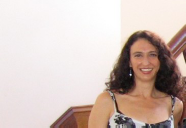
\includegraphics[width=4.7cm]{marcelle_sutton}
\end{minipage}
\begin{minipage}[h]{11.5cm}
\textbf{Marcelle Sutton - Project Manager} \\
Marcelle Sutton studied english and drama and is a qualified teacher.
Marcelle is also a founding member of Linfiniti Consulting CC. - a
small business set up with the goal of helping people to learn and use open
source GIS software. \\
Web: http://linfiniti.com , Email: marcelle@linfiniti.com
\end{minipage}

\vspace{0.1cm}

\begin{minipage}[h]{5cm}
\includegraphics[width=4.7cm]{lerato_nsibande}
\end{minipage}
\begin{minipage}[h]{11.5cm}
\textbf{Lerato Nsibande} \\
Lerato is a grade 12 scholar living in Pretoria. Lerato learns Geography at
school and has enjoyed learning GIS with us!
\end{minipage}

\vspace{0.1cm}

\begin{minipage}[h]{5cm}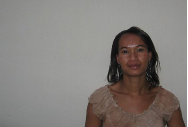
\includegraphics[width=4.7cm]{sibongile_mthombeni}
\end{minipage}
\begin{minipage}[h]{11.5cm}
\textbf{Sibongile Mthombeni} \\
Sibongile lives near Johannesburg with her young daughter. Her goal is to
continue her studies and become a nurse. Working on this project was the
first time Sibongile used a computer.
\end{minipage}
\end{center}
\end{figure}


